%%% TITLE AND AUTHORS %%%%%%%%%%%%%%%%%%%%%%%%%%%%%%%%%%%%%%%%%%%%%%%%%%%%%%%%%
\title[Introduction \& syllabus]{
    Introduction and syllabus \\
    \small{}
}
\author[]{Szymon Talaga and Mikołaj Biesaga} % Your name
\institute[ISS UW]{
    The Robert Zajonc Institute for Social Studies \\ University of Warsaw \\
    \medskip
    \textit{stalaga@uw.edu.pl} \\
    \textit{m.biesaga@uw.edu.pl}
}
\date{2 October 2019} % Date, can be changed to a custom date

%%% SLIDES %%%%%%%%%%%%%%%%%%%%%%%%%%%%%%%%%%%%%%%%%%%%%%%%%%%%%%%%%%%%%%%%%%%%
\frame{\titlepage}

\part[Syllabus]{Syllabus}
\frame{\partpage}

\section[Rules]{Rules of Engagement}
\subsection[Communication]{Communication}
\begin{frame}
    \frametitle{Office Hours, Emails, and Slack}
    \begin{description}[Office Hours:]
        \item[Office Hours:] write us an email or on Slack before coming
        \item[Emails:] the official info will go thorough emails
        \item[Slack:] register at \href{www.slack.com}{www.slack.com}
        \item[Google Drive:] materials and presentations will be posted at \href{https://drive.google.com/a/uw.edu.pl/file/d/1VotLZIEmp4lXnT-NdR0yZ5DDal59FfkI/view?usp=sharing}{Google Drive}
    \end{description}
    \action<visible@+>{\alert{We will try to answer your inquires as soon as possible but do not count on imidiate response, especially before the deadlines.}}
\end{frame}

\subsection[Workflow]{Workflow}
\begin{frame}
    \frametitle{Workflow}
    \begin{enumerate}
        \item Presentation of basic concepts in real-life examples in the classroom.
        \item Exercises in the classroom.
        \item Home assignments requiring modifying the work done in the classroom.
        \end{enumerate}
        \action<visible@+>{\alert{If you cannot find the answer on Internet you are asking the wrong question.}}
    \end{frame}

\begin{frame}
    \frametitle{Stack Overflow}
    \begin{overprint}
        \onslide<+>
            \begin{figure}
                \centering
                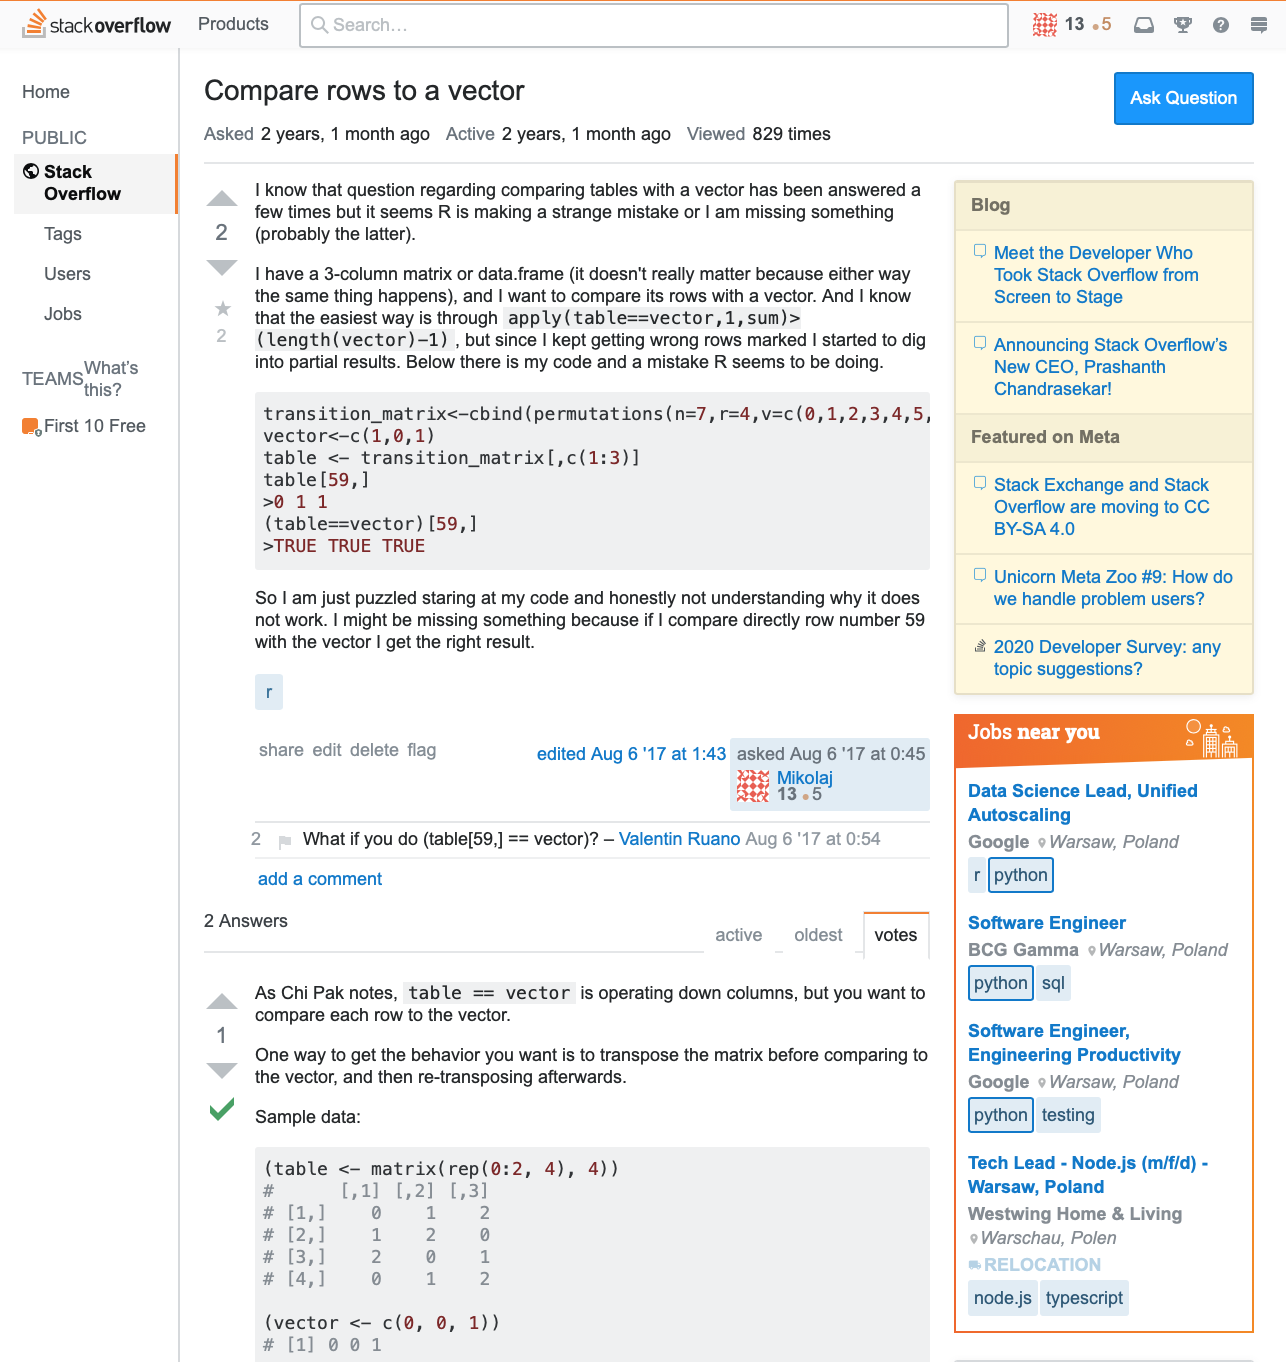
\includegraphics[scale = .3]{png/stack_overflow.png}
            \end{figure}
        \onslide<+>
            \begin{figure}
                \centering
                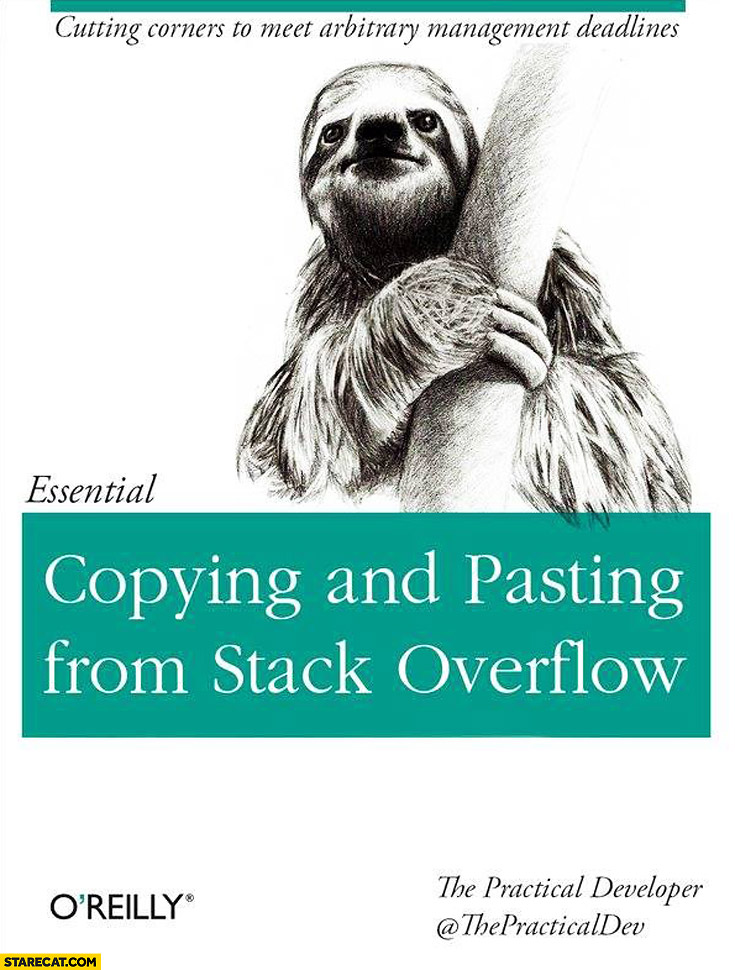
\includegraphics[scale = .175]{png/copy_paste.jpg}
                \caption{from \href{https://xgohorse.com}{https://xgohorse.com}}
            \end{figure}
    \end{overprint}
\end{frame}

\subsection[Assessment]{Assessment Criteria}
\begin{frame}
    \frametitle{Assessment Criteria}
    \begin{block}{}
        Final Grade = 30\%$\times$Homeworks + 35\%$\times$Final Exam + 35\%$\times$written report\\
    \end{block}
        \begin{itemize}
        \item Homeworks - 3 written assignments (approximately after weeks 7, 9, and 13)
        \item Final Exam - will cover theoretical material discussed in the classroom (15.01.2019)
        \item Written Report - a research project proposal formulating a research problem that can be addressed with the methods discussed during the course (due to the last class - 22.01.2019)
    \end{itemize}
\end{frame}

\subsection[Attendance]{Attendance}
\begin{frame}
    \frametitle{Attendance}
    \begin{itemize}
        \item You are allowed to miss up to 2 classes without formal excuse
        \item  absence does not exempt from doing homework assignments
    \end{itemize}
    \action<visible@+>{\alert{It is better not to miss classes because this is a relatively challenging course and it will be hard to cover the material from the class at home.}}
\end{frame}


\part[Introduction]{Introduction}
\frame{\partpage}

\section[CSS]{Computational Social Science}

\begin{frame}
    \frametitle{What is Computational Social Science?}
    \begin{definition}{}
        In the most general sense \emph{Computational Social Science} is a data-driven approach which uses computational methods in studying social phenomena.
    \end{definition}
    \begin{definition}{}
        \emph{Data Science} on the other hand is a broader term than Computational Social Science. It describes the theory and practice of extracting knowledge and insight from data.
    \end{definition}
\end{frame}

\begin{frame}{General interest in data science}
    \begin{figure}
    \setbeamertemplate{caption}
    \caption{Growth of Google search}
    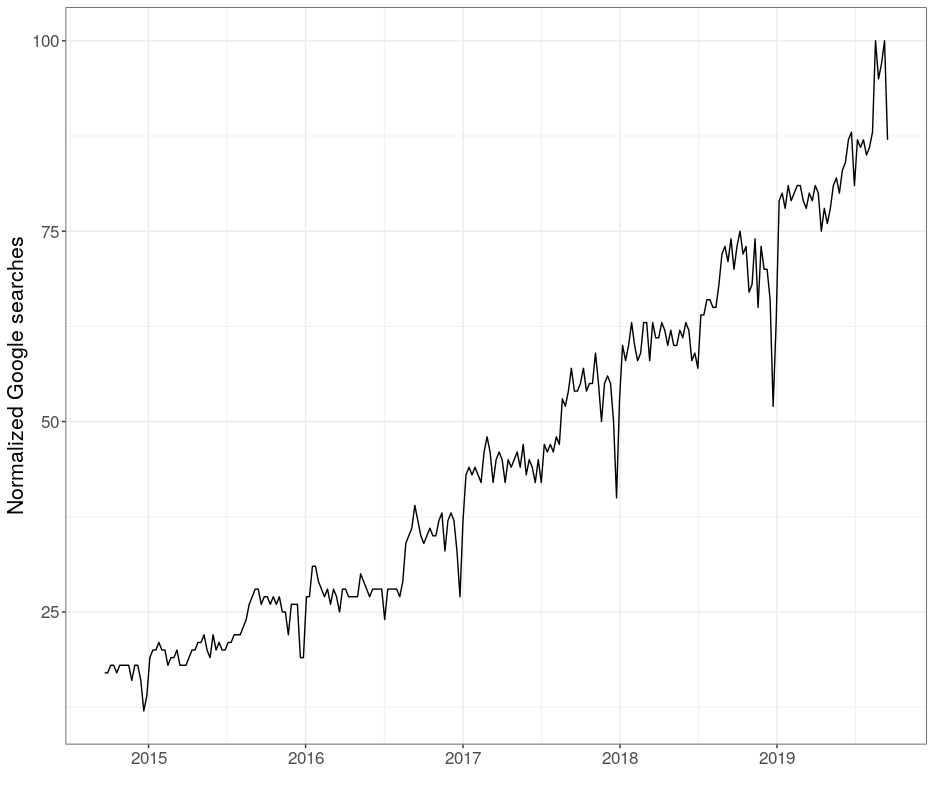
\includegraphics[width = .8\framewidth]{png/ds-searches.png}

    \end{figure}
\end{frame}

\subsection{Research Methods}

\begin{frame}
    \frametitle{Traditional Research Methods}
        \only<1>{
            Tutaj będzie schemat tradycyjnych badań psychologicznych
        }
        \only<2>{
            \begin{itemize}
                \item surveys
                \item observational studies
                \item experiments
                \item case studies
                \item event sampling methodology (diaries)
                \item interviews
                \item meta-analysis
            \end{itemize}}
        \only<3>{
            \resizebox{\textwidth}{!}{
                \begin{tabular}{l | c | c | c | c | c | c }
                Id & Sex & Age & Condition & Variable A & Variable B & Variable C\\
                \hline \hline
                AAA & M & 24 & exp & 55:53 & 3 & apple\\
                AAB & F & 22 & exp & 53:47 & 2 & banana\\
                AAC & F & 28 & con & n/a   & 4 & banana\\
                AAD & M & 21 & con & 54:35 & 3 & banana
                \end{tabular}}
        }
\end{frame}

\begin{frame}
    \frametitle{Computational methods}
    \setbeamercovered{transparent}
    \begin{itemize}
        \item<1> extraction of unstructured data from external digital (i.e. web-based) sources
        \begin{itemize}
            \item<1> webscraping (extraction of data from existing webpages)
            \item<1> extracting data from web APIs (i.e. Twitter)
        \end{itemize}
        \item<1> analysis of textual data (natural language processing - NLP)
        \item<0> network and relational data analysis
        \item<0> working with big datasets (that do not fit into RAM of a single computer), in-database computations, distributed computing etc.
        \item<0> computer simulations
        \item<0> online experiments (A/B testing, experiments based on online games etc.)
    \end{itemize}
\end{frame}

\section[Data]{Data}

\subsection[Data Sources]{Data Sources}
\begin{frame}
    \setbeamercovered{transparent}
    \frametitle{Data Sources}
    \only<1>{
        \begin{figure}
            
\includegraphics[scale=.35]{png/data_everywhere.png}
        \end{figure}}
    \only<2>{
        \begin{itemize}
            \item<2> social media
            \item<2> web pages
            \item<0> smart devices
            \item<0> digital behavioral data
            \item<0> mobile phone networks
            \item<0> goverment data
            \item <0>...
        \end{itemize}
        \action<2>{\alert{The fact that you can get the data does not mean you should.}}
    }
\end{frame}

\subsection{Webscraping}

\begin{frame}
    \frametitle{Webscraping}
    \only<+>{
        \begin{figure}
            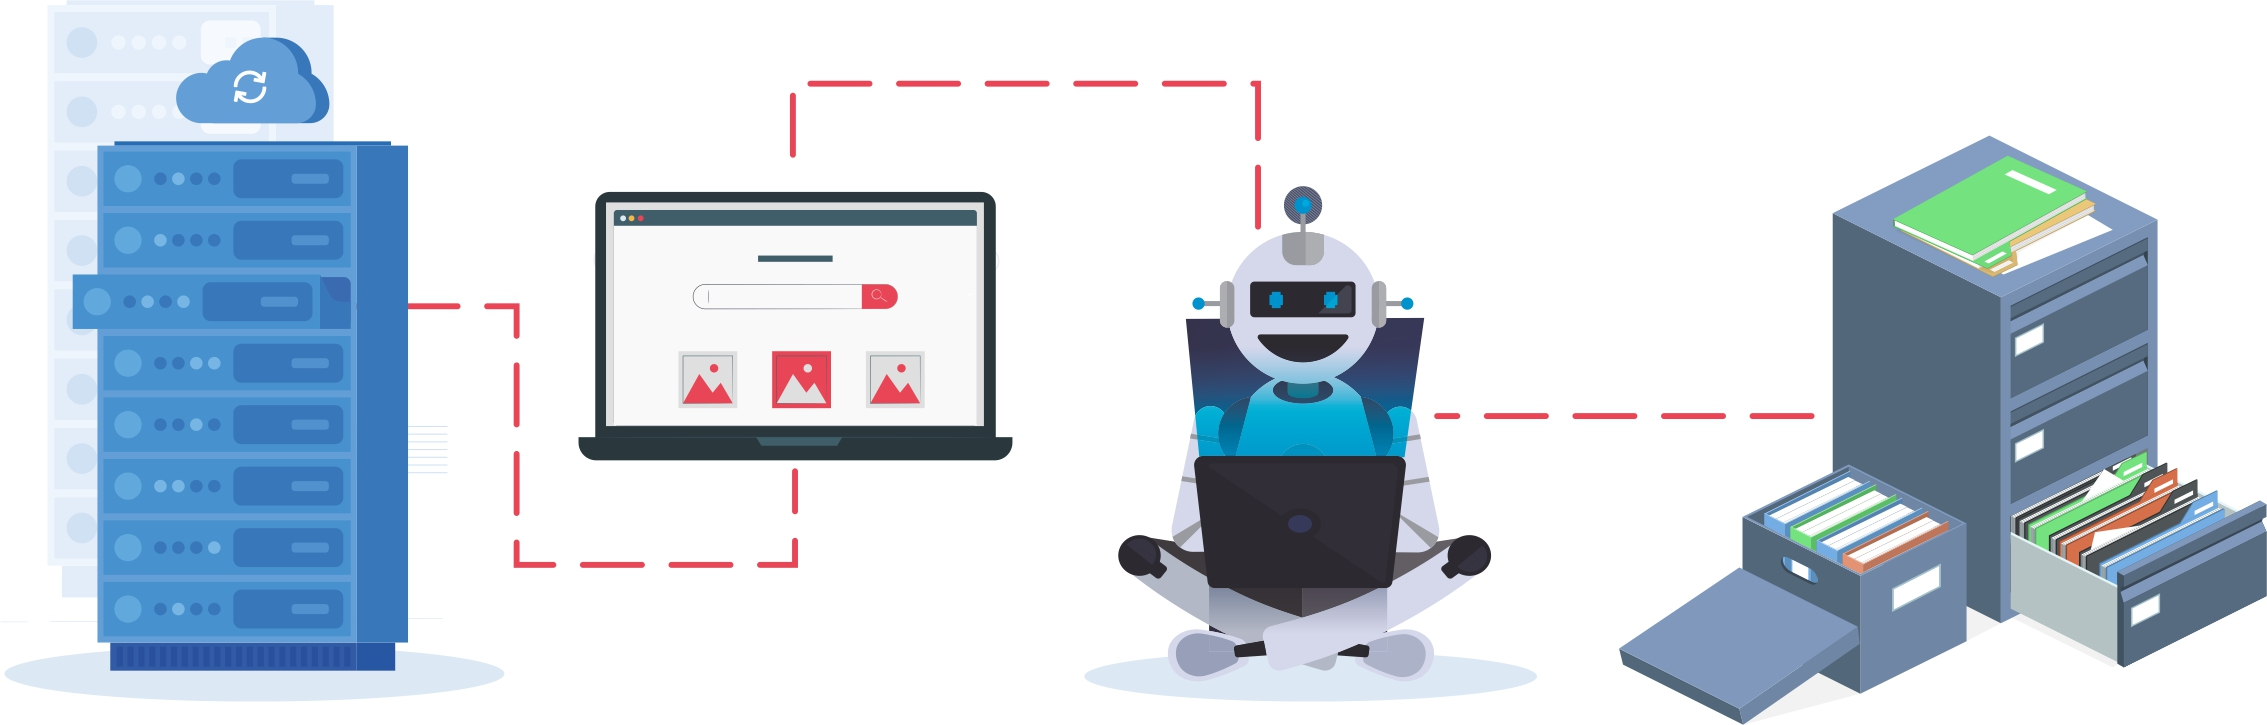
\includegraphics[scale = .15]{png/webscraping.jpg}
            \caption{from \href{https://www.edureka.co/}{https://www.edureka.co/}}
        \end{figure}
    }
    \only<+>{
        \begin{figure}
            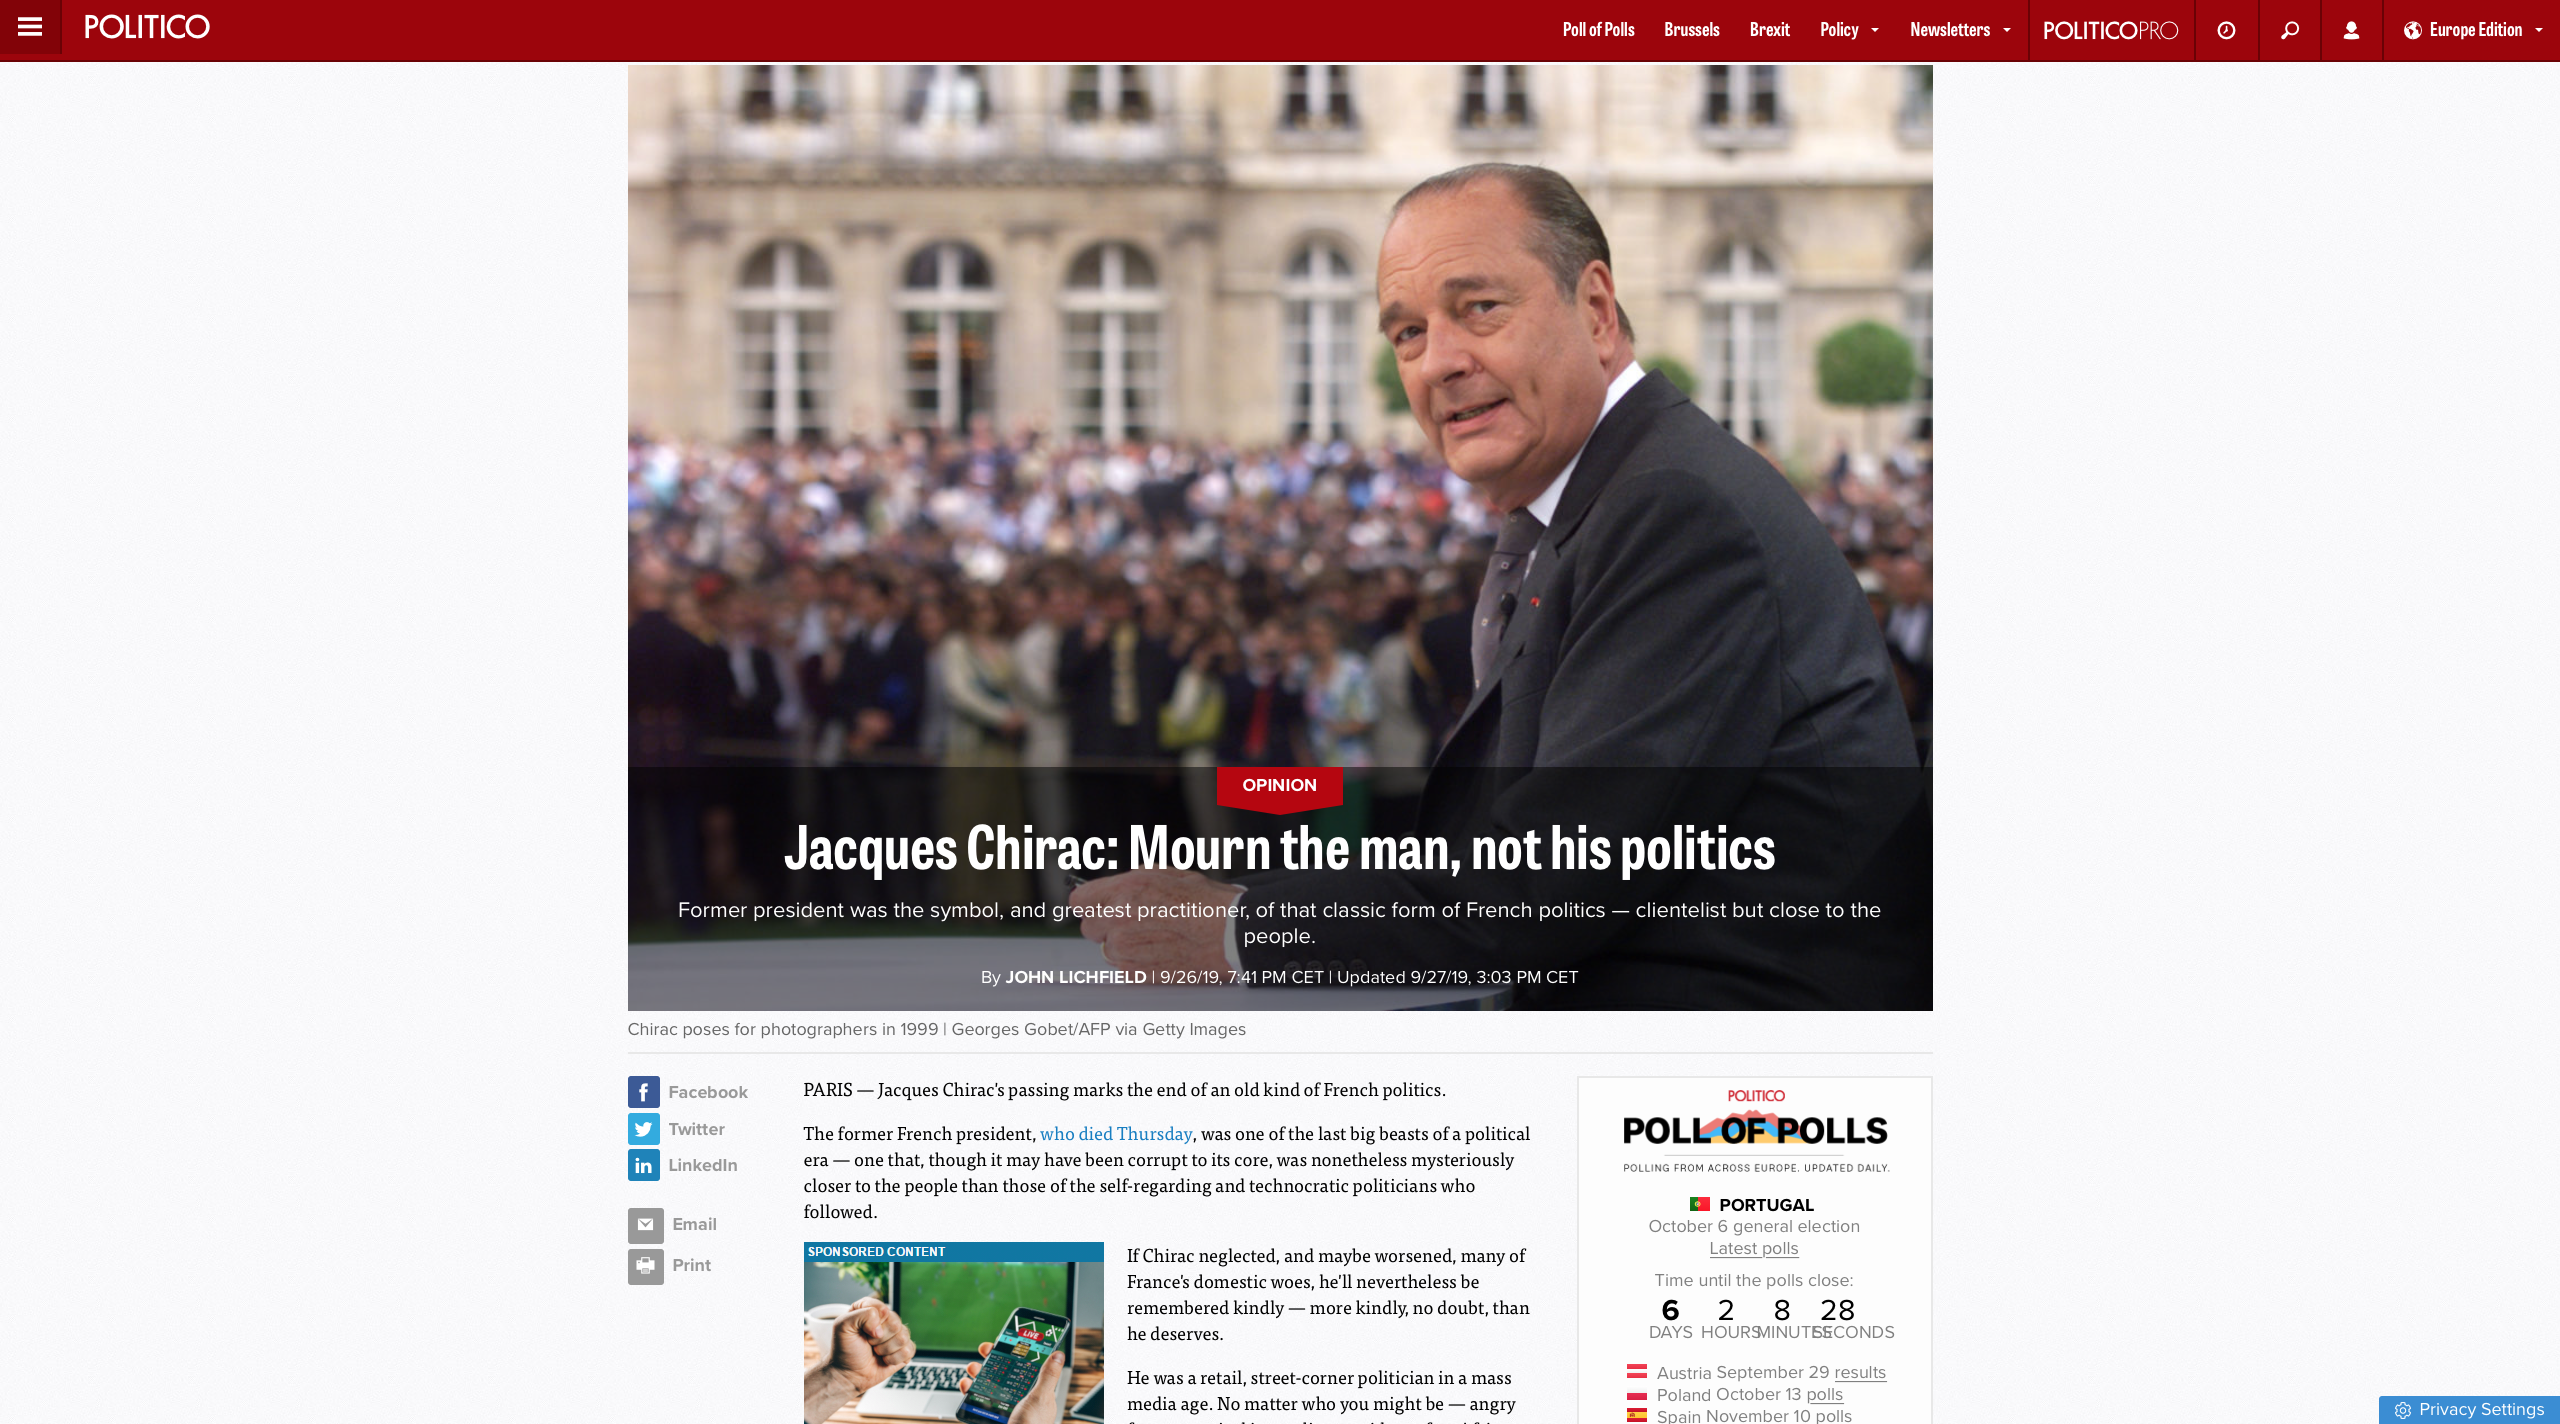
\includegraphics[scale = .22]{png/politico.png}
            \caption{from \href{https://www.politico.eu/article/jacques-chirac-mourn-the-man-not-his-politics/}{POLITICO Europe}}
        \end{figure}
    }
    \only<+>{
        \begin{definition}
            \emph{Webscraping} is a process of (usually) automatic extraction of data from a website or multiple websites. In other words, it is a form copying the data from a website into a local database or spreadsheet.
        \end{definition}
    }
\end{frame}

\subsection{API}

\begin{frame}
    \frametitle{Application Programming Interface}
    \only<+>{
        Tutaj będzie schemat tego co to jest API
    }
    \only<+>{
        \begin{figure}
            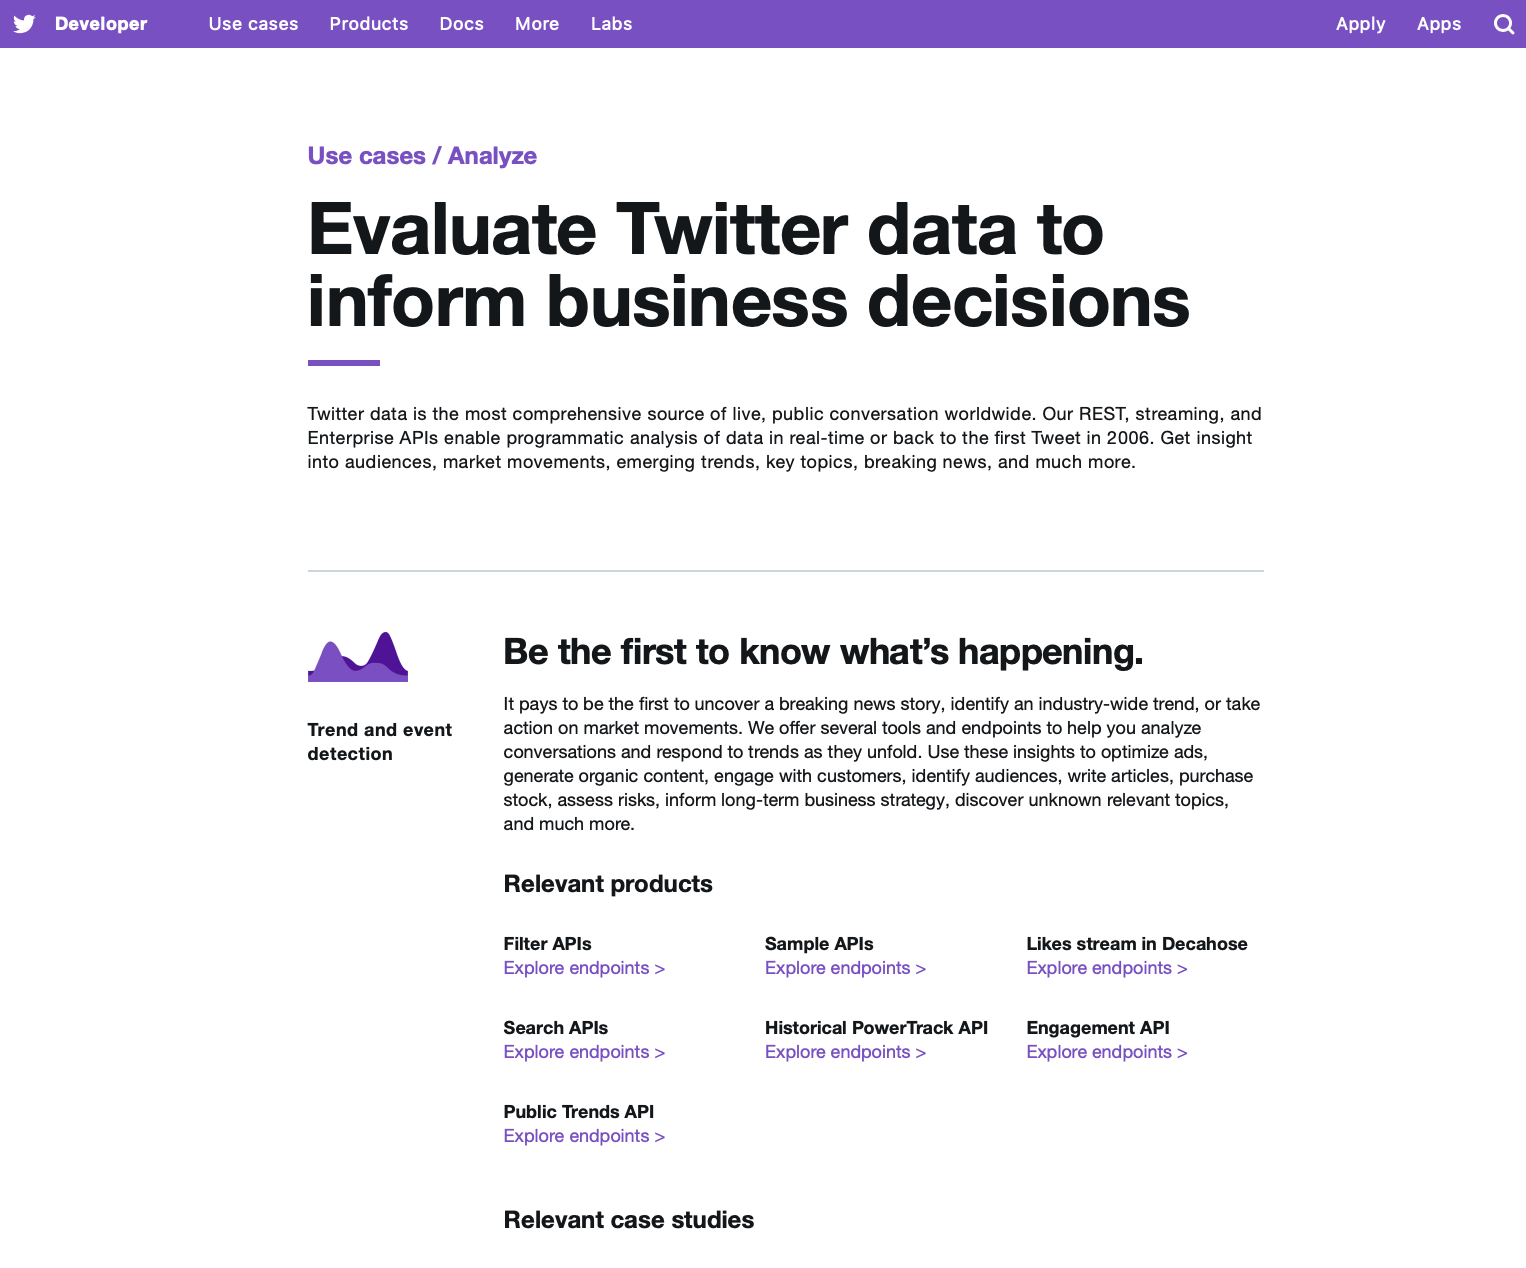
\includegraphics[scale =.3]{png/twitter.png}
            \caption{from \href{https://developer.twitter.com/en/use-cases/analyze}{Developer Twitter}}
        \end{figure}
    }
    \only<+>{
        \begin{definition}
            \emph{Aplication Programming Interface} is a communication protocol between a client and a server intended to simplify the building of client-side software. In other words, it is a contract between the client and the server which defines the format of possible requests and format of the response (i.e. format of the data).
        \end{definition}
    }
\end{frame}

\subsection[Data Formats]{Data Formats}

\begin{frame}
    \frametitle{Structured and Unstructured data}
    \only<1>{
        Tu wstawić obrazek z uporządkowaną szafką i z drugiej strony z bałaganem
    }
    \only<2>{\begin{columns}[t]
        \begin{column}{.5\textwidth}
            Structured Data:
            \begin{itemize}
                \item can be displayed in rows and columns
                \item numbers, text, dates
                \item requires less storage
                \item easy to manage and analysis
            \end{itemize}
        \end{column}
        \begin{column}{.5\textwidth}
            Unstructured Data:
            \begin{itemize}
                \item can't be displayed in rows and columns
                \item images, audio, video, e-mails, spreadsheets etc. (fun staff)
                \item requires more storage
                \item extremely hard to manage and analysis
            \end{itemize}
        \end{column}
    \end{columns}}
\end{frame}

\begin{frame}[fragile]
    \frametitle{JSON - JavaScript Object Notation}
    \defverbatim[colored]\mycode{%
        \begin{lstlisting}[
            frame=single,
            language=json,
            firstnumber=1,
            basicstyle=\footnotesize\ttfamily
        ]
        { name: "Alice",
          age: 17,
          interests: [
            { name: "sport",
              tags: [
                "physical activity",
                "outdoor"
            ] }
        \end{lstlisting}
    }
    \mycode
    \begin{definition}
        \emph{JavaScript Object Notation} is a lightweight text data format which is relatively easy to read for both human naked eye and computers. Although it derives from JavaScript it is a language-independent data format. JSON is built on two structures: a collection of key-item pairs and ordered list of values. JSON filenames use .json extension.
    \end{definition}
\end{frame}


\begin{frame}[fragile]
    \frametitle{JSON Lines}
    \defverbatim[colored]\mycode{%
        \begin{lstlisting}[
            frame=single,
            language=json,
            firstnumber=1,
            basicstyle=\footnotesize\ttfamily
        ]
        {name:"Alice","favorite fruit":["plums","grapes"]}\n
        {name:"Bob","favorite fruit":["watermelons"]}
        \end{lstlisting}
    }
    \mycode
    \begin{definition}
        \emph{JSON Lines} (newline-delimited JSON) is a lightweight text data format which can be processed one record at a time. Each line consists of a JSON. JSON Lines filenames use .jl or .jsonl extensions.
    \end{definition}
\end{frame}

\section[NLP]{Natural Language Processing}

\begin{frame}
    \frametitle{Natural Language Processing}
    \only<+>{
        Tutaj będzie schemat NLP
    }
    \only<+>{
        \begin{definition}
            In general sense \emph{Natural Language Processing} (NLP) is an analytical approach which uses set of (usually) computer-based methods to extract meaning, topics or sentiment from natural language data (written or spoken). In other words, it is a set of computer algorithms which tries to synthesize human language.  \end{definition}
    }
    \only<+>{
        \begin{itemize}
            \item tokenization
            \item stemming
            \item lemmatization
            \item sentiment analysis
            \item vector models
            \item topic modeling
            \item part of speech tagging
            \item entities analysis
    \end{itemize}
    }

\end{frame}

\section[One more things]{One more thing...}
%%% LITERATURE %%%%%%%%%%%%%%%%%%%%%%%%%%%%%%%%%%%%%%%%%%%%%%%%%%%%%%%%%%%%%%%%
\begin{frame}
    \frametitle{Literature to read}
    \nocite{*}
    \AtNextBibliography{\footnotesize}
    \printbibliography
\end{frame}


\note{
    https://www.theguardian.com/us-news/2015/dec/11/senator-ted-cruz-president-campaign-facebook-user-data
}
